\chapter{Pricing: Learning the Best Price}

Design a learning algorithm for pricing when the users that will buy the product are those that have clicked on the ads. Assume that the allocation of the budget over the three subcampaigns is fixed and there is only one phase (make this assumption also in the next steps). Plot the cumulative regret.

\section{Demand Curves}

\begin{figure}[hp]
	\centering
	%\captionsetup{justification=centering,margin=1cm}

	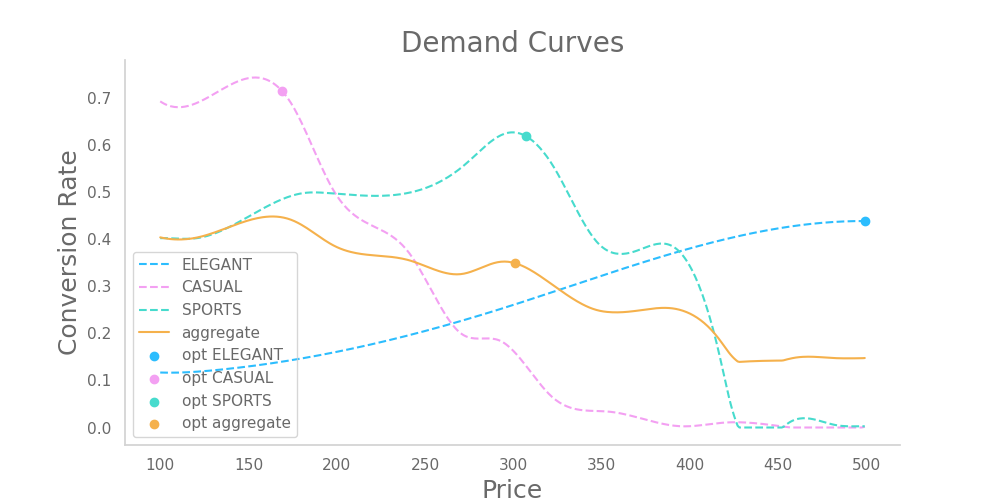
\includegraphics[width=1.0\textwidth]{images/demand_curves.png}
	\caption{\textbf{Demand Curves}.\\
		It used to show the probability (\textit{conversion rate}) that a certain class, of customers, will buy or not the product w.r.t. a proposed price.\\
		The dashed lines represent the demand curves of the corresponding classes:
		\textit{blue} for the \textit{Elegant} class;
		\textit{pink} for the \textit{Casual} class; and
		\textit{light green} for the \textit{Sports} class.\\
		The \textit{orange} curve is the mean between the others and it is used to study the \textit{aggregate} model.\\
		The points are displayed to show the optimal price w.r.t. the conversion rate: the area below them is maximum.}
		\label{demandCurvesFig}
\end{figure}

\section{Environment}

\section{Learner Algorithm Selection}

\section{Experiments}

\section{Results}

\begin{figure}[!htb]
	\centering
	%\captionsetup{justification=centering,margin=1cm}
	
	\begin{subfigure}[!H]{0.8\textwidth}
		\centering
		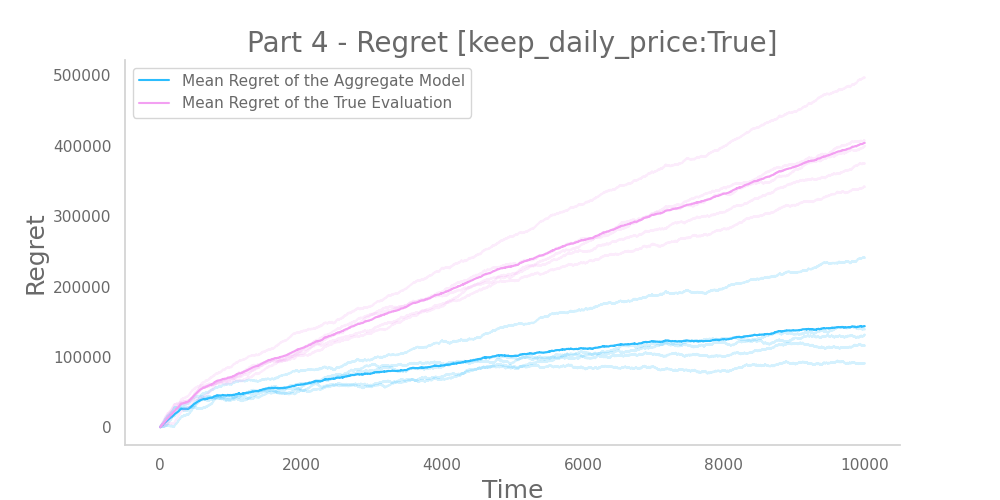
\includegraphics[width=\textwidth]{images/part4_keep-daily-priceTrue.png}
		\caption{Regret obtained proposing to the customers the same price for the entire day.}
	\end{subfigure}
	%\hfill
	\begin{subfigure}[!H]{0.8\textwidth}
		\centering
		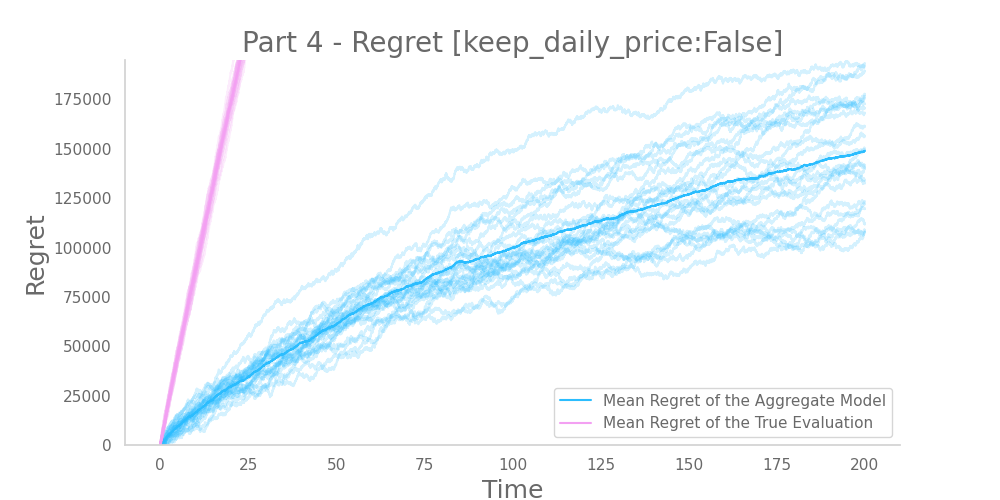
\includegraphics[width=\textwidth]{images/part4_keep-daily-priceFalse.png}
		\caption{Regret obtained proposing to the customers different prices for each visit. This method achieves better performances since the learner collects more data during the campaign.}
	\end{subfigure}

	\caption{Comparison between the regrets obtained after the campaign.\\
			The \textbf{Mean Regret of the Aggregate Model} (colored in \textit{blue}) is the regret computed keeping, as optimal, the area under the optimal point of the aggregate curve~\ref{demandCurvesFig}. In other words, both the learner and the clairvoyant don't know the class of the customers. This is an optimistic measure of the regret.\\
			The \textbf{Mean Regret of the True Evaluation} (colored in \textit{pink}) is the regret obtained computing the optimal value exploiting the original class of the customers.}
\end{figure}